\documentclass[11pt]{book}

\usepackage[authoryear]{natbib}
\usepackage{xcolor}
\usepackage[T1]{fontenc}
\usepackage{fourier}
\usepackage[utf8]{inputenc}
\usepackage[hidelinks]{hyperref}
\usepackage{slashbox}
\usepackage{graphicx}
\usepackage{url}
\usepackage{enumitem}
\usepackage[font=small,labelfont=bf]{caption}
\usepackage{float}
\usepackage{amsmath}
\usepackage{algpseudocode}
\usepackage{algorithm2e}

\newcommand{\todo}[1]{\textcolor{red}{[TODO: #1]}\PackageWarning{TODO:}{#1!}}
\newcommand{\note}[1]{\textcolor{red}{[NOTE: #1]}\PackageWarning{NOTE:}{#1!}}
\newcommand*{\np}{\par\noindent\newline}

\title{Agent Based Models of the Formation of Social Preferences}
\author{S Pardy}
\begin{document}
\begin{titlepage}
	\newcommand{\HRule}{\rule{\linewidth}{0.5mm}} % Defines a new command for horizontal lines, change thickness here
	
	\center % Centre everything on the page
	
	%------------------------------------------------
	%	Headings
	%------------------------------------------------
	
	\textsc{\LARGE Monash University}\\[1.5cm]	
	\textsc{\Large Bachelor of Science (Honours)}\\[0.5cm] % Major heading such as course name
	
	\textsc{\large Computational Science}\\[0.5cm] % Minor heading such as course title
	
	%------------------------------------------------
	%	Title
	%------------------------------------------------
	
	\HRule\\[0.4cm]
	
	{\huge\bfseries Agent Based Models of the Formation of Social Preferences}\\[0.4cm]
	
	\HRule\\[1.5cm]
	
	%------------------------------------------------
	%	Author(s)
	%------------------------------------------------
	
	\begin{minipage}{0.4\textwidth}
		\begin{flushleft}
			\large
			\textit{Author}\\
			Sam \textsc{Pardy}
		\end{flushleft}
	\end{minipage}
	~
	\begin{minipage}{0.4\textwidth}
		\begin{flushright}
			\large 
			\textit{Student ID}\\
		25940783   
		\end{flushright}
	\end{minipage}
	\vfill
	\vfill
	{\large
	\textit{Supervisor}\\
	Dr. Julian \textsc{Garcia}}
	
	%------------------------------------------------
	%	Date
	%------------------------------------------------
	
	\vfill\vfill\vfill % Position the date 3/4 down the remaining page
	
	{\large\today} % Date

	\vfill % Push the date up 1/4 of the remaining page
	
\end{titlepage}
% \hypersetup{colorlinks, citecolor=black, filecolor=black, linkcolor=black urlcolor=black}

% \newpage
% \chapter*{Declaration}
% \chapter*{Abstract}
% \chapter*{Acknowledgment}

\tableofcontents
\newpage
\listoffigures
\chapter{Introduction}
\section{Preamble}
\section{Motivation \& Objectives}

\chapter{Literature Review}

\section{Limitations of Theory}
The theoretical and analytical work discussed in the previous chapters suffers from several limitations that affect the generality of the conclusions drawn. 
Chiefly, it is static; the conclusions focus on evolutionary stable strategies as a solution concept.
These conclusions may be meaningful however do not tell us anything about how likely these strategies are to evolve or what circumstances may lead to them evolving.
Further, the work is slightly abstract in that in places it does not detail specific attributes of the model it is working with in favour of broader `catch-all' definitions,
this has made the process of creating simulation-based models of the theory difficult at times.

\np The primary source of theoretical work that this research has been on based is that of Alger \& Weibull (\citeyear{alger_generalization_2012}, \citeyear{alger_homo_2013}; henceforth, \textit{AW}).
This work finds that under certain assumptions a utility function that is centred around a linear relationship between the two players' payoffs results in evolutionarily stable play.
This utility function is given in equation \ref{linearESSEquation}, in which \textit{x} and \textit{y} are types in the population and $\alpha$ is equal to the \textit{index of assortativity}.
\begin{equation}
	\label{linearESSEquation}
	u_\alpha(x, y) = \Pi(x,y) + \alpha\Pi(y,x)
\end{equation}

\noindent To achieve this, the authors assume that all types have a utility function of the same form as \ref{linearESSEquation} where $\alpha \in (-1, 1)$ \citep[p. ~47]{alger_generalization_2012}.
With this assumption, the model, in essence, only allows one number ($\alpha$) to freely evolve.
This assumption severely limits the search space of the evolutionary process. 
The experimental framework that we have created relaxes this assumption.

\np A further assumption made in AW is that while players do not have information about their opponent's preferences,
the players converge to "mutually compatible" strategies and, in effect, play a Nash equilibrium with perfect information \citep[p. ~46]{alger_generalization_2012}.
It is unclear how realistic this assumption is. 
As discussed in previous chapters, it does not make sense to assume that players have knowledge about their opponent's preferences 
but it may be acceptable to assume that when engaging in repeated interactions players converge to Nash equilibrium play relatively quickly.
It is possible, though, that this assumption impacts the evolutionarily process substantially. 
Our experimental framework relies on this assumption also.

\np Commonly in the literature it is assumed that the agents will be matched to play symmetric, two-player games.
This is true also of \citet{alger_generalization_2012}.
In general, a \textit{symmetric} two-player game entails that an agent is indifferent (in terms of payoffs) as to which of the players she takes the roles of in the interaction.
This assumption makes easier our job of implementing a fitness-comparison mechanism.
As fitness is linked to the respective payoff achieved by each agent, the fact that the net payoff on offer to each player is equal simplifies the eventual fitness comparison.
However, we will see later that this assumption may have contributed to some bias in the sampling.

\np A final assumption to note is that the fitness used in the model in \citet{alger_generalization_2012} is that of \textit{average} fitness.
This measure is less stringent than measures used elsewhere (notably in \citet{alger_homo_2013}). 
An oft used fitness measure requires that for an invasion to occur, a mutant must achieve a higher payoff in all equilibria of all games the two types play when they're matched.

\np Of course, these assumptions are all made within the context of a model that is static.
The conclusions drawn in the work referenced above tend to be of the form \textit{should} a utility function of the form \textit{x} evolve it will result in evolutionary stable play given the assumptions.
The experimental framework we create intends to investigate these conclusions and assumptions in a dynamically evolving environment.
The experimental framework that we have created as part of \textit{this} research seeks to recreate these models as dynamically-evolving before attempting to recover the results achieved in existing, static work.

\todo{Why static v dynamic important? => eq selection, dynamics, diversity}
\todo{emphasise how big an assumption static is}





\chapter{The Experimental Framework}\label{experimentalFramework}
A large part of the work undertaken in support of this research involved the creation of an experimental framework that could be used to attempt to recover the results of \citet{alger_generalization_2012} in a dynamically evolving environment.
At a high level this experimental framework is simple, however when digging into the detail, complications arise.
Fundamentally, the framework is made up of a representation of a utility function, 
a means by which instances of this representation can be mutated and a means by which the fitness of two different utility functions can be compared.
With these building blocks we can construct the main loop of the experiments that are undertaken.
We define some utility function that represents our initial resident agent, the resident is then mutated (creating the mutant). 
The fitnesses of both resident and mutant are then computed and compared. 
If the mutant achieves a higher payoff an invasion occurs: the original resident is discarded and the mutant takes over as the new resident.
This process is repeated for a given number of generations.
In the following, we discuss the implementation detail of each of these fundamental parts of the framework, beginning with fitness.


\section{Fitness}
\np Decisions we make about how we measure fitness and what difference in fitness is enough to trigger an invasion can have significant impact on the dynamics of the system.
This is an area in which Alger \& Weibull give us limited but essentially sufficient guidance.
Fitness is measured as the \textit{personal payoff} earned by each type when both players act in accordance with their own preferences.
For an individual $\theta$ in a population state $(\theta, \theta', \epsilon,\sigma)$,
where $\theta'$ is the mutant, $\epsilon$ is the mutant share of the population and $\sigma$ is the \textit{index of assortativity}, the expected fitness gain of the resident and mutant after one interaction is given by equations \ref{FexpectedPayoff} \& \ref{GexpectedPayoff} respectively.
Where $f(x, y)$ is the expected payoff earned by $x$ when facing $y$ in a given interaction.
\newline
\begin{gather}
	\label{FexpectedPayoff}
	F_{\epsilon, \sigma}(\theta, \theta') = (\sigma +(1-\epsilon)(1-\sigma))f(\theta, \theta) + \epsilon(1-\sigma)f(\theta, \theta')\\
	\label{GexpectedPayoff}
	G_{\epsilon, \sigma}(\theta', \theta) = (\sigma +\epsilon(1-\sigma))f(\theta', \theta') + (1-\epsilon)(1-\sigma)f(\theta', \theta)
\end{gather}

\np The notion of evolutionary stability is defined as follows: for a state to be considered stable, the residents must achieve, \textit{on average}, a fitness at least as high as that achieved by the mutants in a population that contains both resident and mutant types.
Using functions \ref{FexpectedPayoff} and \ref{GexpectedPayoff}, this relation is given by \ref{ESSweakInequality}.
\begin{equation}
	\label{ESSweakInequality}
	F_{\epsilon, \sigma}(\theta, \theta') \geq G_{\epsilon, \sigma}(\theta', \theta)
\end{equation}
\citet[~p. 44]{alger_generalization_2012}
\np So, if inequality \ref{ESSweakInequality} does not hold, an invasion occurs.

\begin{figure}[H]
	\centering
	\begin{algorithm}[H]
		\KwData{$\theta$, $\theta'$}
		\KwResult{fitness of $\theta$}
		thetaFitness = 0\;
		\For{specified number of games}{
		 randomly sample payoffs to create new \textit{payoffGame}\;
		 transform \textit{payoffGame} using both individual's utility functions to create \textit{utilityGame}\;
		 \For{each equilibrium in utilityGame}{
		  increase \textit{thetaFitness} by the expected payoff of playing \textit{equilibrium} in \textit{payoffGame}\;
		 }	   
		}
		return (thetaFitness $\div$ number of equilbria in \textit{utilityGame}s)\;
	   \end{algorithm}
	\caption{Pseudocode for the algorithm to perform a fitness comparison.}
	\label{psuedocodeForf}
\end{figure}

\np The place where we are left to make some of our own decisions regarding fitness is in deciding what constitutes the expected payoff function, $f(x,y)$.
Since the authors assume that an \textit{average} payoff is used, the expected payoff function is implemented as the average expected payoff across all equilibria, across all games that individuals play in a given interaction.
Figure \ref{psuedocodeForf} shows a pseudocode for the function $f$.

\np This discussion of expected payoff raises the question of the kinds of games that will be played in these interactions - this is the topic of our next discussion.

\begin{figure}[H]
	\vspace{30px}
	\centering
	\begin{tabular}{|l||*{5}{c|}}\hline
		\backslashbox{Player A}{Player B}
		&\makebox[7em]{Action 1}&\makebox[7em]{Action 2}\\\hline\hline
		Action 1 & a, a & b, c\\\hline
		Action 2 & c, b & d, d \\\hline
	\end{tabular}
	\caption{Payoff matrix detailing the payoff structure of a symmetric game. Where Player A earns the payoff on the left of the cell, and Player B the payoff on the right, and ${a, b, c, d} \in R$.}
	\label{symmetricGame}
	\vspace{20px}
\end{figure}
\section{Games}
\np A key part of any game-theoretic model that attempts to represent the process of preference formation, is the kinds of games that are played.
For the most part, the literature (\citet{alger_generalization_2012}, \citet{alger_homo_2013}, \citet{newton_preferences_2017}) is largely agnostic about the games that are played in the models the work describes.
This work assumes only that the games are symmetric and two player. 
With this assumption in mind, \ref{symmetricGame} shows the payoff structure of a symmetric game.

\np Given that we are interested in how cooperative preferences can develop, we begin with a model in which individuals are matched to play a single type of non-cooperative game.
For example, using a prisoner's dilemma type we can write down a game with the payoff structure detailed in figure \ref{symmetricGame} with payoffs $c > a > d > b$.
Next, we investigate how preferences form when individuals play many different symmetric games in one interaction.
Now, the payoffs $a$ through $d$ are determined as follows:

\begin{center}\label{a_through_d}	
$a \sim U(0,\phi) \qquad a \in I$

$b \sim U(0,\phi) \qquad b \in I$

$c \sim U(0,\phi) \qquad c \in I$

$d \sim U(0,\phi) \qquad d \in I$
\end{center}

\np In other words, $a, b, c, d$ are independent and identically distributed uniform random variables from $0$ to some maximum $\phi$.

\np \todo{Might say something about asymmetric games here}

\np In Chapter \ref{symmetricGames} we discuss results relating to both single- and many-game interactions.


\section{Representing \& Mutating Individuals}
\np The way that utility function types are mutated is intrinsically tied to way that those types are represented in the framework, so we will here discuss them together.
Fundamentally, a utility function in this context is a way to convert the outcomes experienced by two individuals into the utility of one of those individuals.
The individual then acts so as to maximize their utility, and in this way acts like an individual who \textit{prefers} strategy $x$ to strategy $x'$ \textit{iff} $u(x, y) > u(x', y)$.
The experimental framework we setup explores the way two methods of representing individuals affects the dynamics of the system.
The first method involves maintaining the values of a `utility surface' directly. 
While the second, style of representation involves maintaining a two parameter function $f(x,y)$, where x is the payoff earned by the agent whose utility function $f$ is and y is the payoff earned by their opponent. 
Both methods will be examined in detail in the following.


So, an individual is represented as a matrix of utility values that can be queried by payoff.
Mutation is performed by making small, localised changes to an area of the surface.
The second 


\paragraph{Phenotype Mutation}
\np The method by which individuals are represented as utility surfaces we've termed `phenotype mutation'.
This is because in this method individuals are represented directly as a surface in 3 dimensions.
So the only information maintained about different types is their phenotype and mutation is performed directly on the phenotype.
The three dimensions of the surface (from the individuals point of view) are: my payoff, my opponent's payoff, and my utility.
Figure \ref{selfishUtilitySurface} is an example of a purely selfish utility surface.

\np This method has two immediate limitations. 
The first is that the surface is only defined for a certain payoff range and so a value, $\phi$ must be provided that represents the maximum \textit{payoff} achievable by either individual.
Second, the surface is discretised and so is accurate only up to a certain granularity - a value, $s$ must be provided that is the `step' of the grid.
The value $s$ should be as small as feasible. 
Figure \ref{selfishUtilityGrid} is an example of the grid values of a utility surface of an individual that is purely selfish.

\begin{figure}
	\centering
	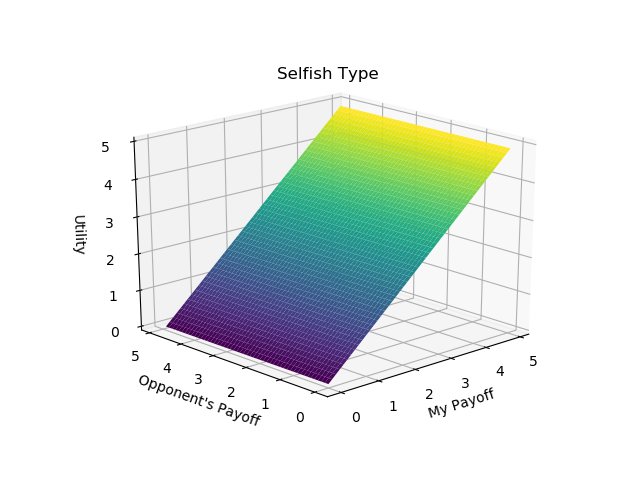
\includegraphics[scale=0.75]{resources/selfish.png}
	\caption{An example of a purely selfish type represented as a `utility surface'.}
	\label{selfishUtilitySurface}
\end{figure}

\begin{figure}
\[
	\begin{bmatrix} 
	0. & 0. & 0. & \dots & 0. & 0. & 0.\\
	0.1 & 0.1 & 0.1 & \dots & 0.1 & 0.1 & 0.1\\
	0.2 & 0.2 & 0.2 & \dots & 0.2 & 0.2 & 0.2\\
	\vdots & \vdots & \vdots & \dots & \vdots &\vdots &\vdots\\
	4.7 & 4.7 & 4.7 & \dots & 4.7 & 4.7 & 4.7\\
	4.8 & 4.8 & 4.8 & \dots & 4.8 & 4.8 & 4.8\\
	4.8 & 4.8 & 4.8 & \dots & 4.8 & 4.8 & 4.8 
	\end{bmatrix}
\]
\caption{A `selfish' utility grid with $\phi = 5$ and $s = 0.1$.}
\label{selfishUtilityGrid}
\end{figure}

\np Phenotypic mutation is performed by creating a small perturbation to the resident surface in a randomly selected area.
We assume this perturbation takes the shape of a bivariate normal distribution with standard deviation $\sigma$, where $\sigma \sim U(0,\gamma)$ and $\gamma$ is a parameter of the model.
This method ensures that mutations are small.
It also has the effect of creating \textit{localised} mutations: mutations that only affect a certain area of the surface rather than the shape of the surface overall.
It turns out that the localised nature of these mutations is important and will be discussed in proceeding sections.
Figure \ref{selfishUtilitySurfaceOneMutation} shows our selfish utility surface from \ref{selfishUtilitySurface} after one mutation has been applied.
\begin{figure}
	\centering
	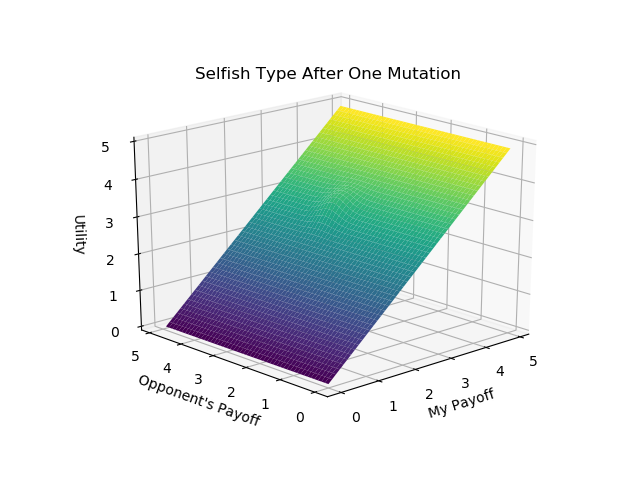
\includegraphics[scale=0.7]{resources/one_mutation.png}
	\caption{The selfish utility surface after one mutation has been applied at the point (3, 3).}
	\label{selfishUtilitySurfaceOneMutation}
\end{figure}
\paragraph{Symbolic Regression}
\np The second method by which we represent individuals is by maintaining the symbolic expression of a two parameter function.
This expression (which is the phenotype) is not the only information stored about each individual though.
An individual also consists of its genome, an array of integers (`codons') that is used to generate the phenotype in conjunction with the grammar.
This representation uses the work of \citet{fenton_ponyge2:_2017}, the documentation of which has in depth explanations of the representation's inner workings.

\np Briefly, the grammar is a set of rules that govern the kinds of individuals that can be generated.
To generate a phenotype, the grammar rules are enumerated with the phenotype iteratively constructed.
Each time a choice is to be made between two or more options, we take the modulo of the current codon by the number of available options, this value is used to select the rule.
The grammar, in Backus-Naur form \citep{oneill_grammatical_2001}, is a parameter of the model and inherently introduces bias into the simulation.
The grammar that was used for the majority of our simulations is shown in \ref{grammar}, where $<o>, <e> and <c>$ are rules and the terms separated by $|$ are the possible results of that rule.

\begin{align}\label{grammar}
	&<o> ::= \qquad <e>+<e>|\\
	& \qquad \qquad \qquad <e>-<e>| \nonumber \\
	& \qquad \qquad \qquad <e>*<e>| \nonumber \\ \nonumber \\
	&<e> ::= \qquad <e>+<e>| \nonumber \\
	&\qquad \qquad \qquad <e>-<e>| \nonumber \\
	&\qquad \qquad \qquad <e>*<e>| \nonumber \\
	&\qquad \qquad \qquad <c><c>.<c><c>| \nonumber \\
	&\qquad \qquad \qquad r| \nonumber \\
	&\qquad \qquad \qquad myPayoff| \nonumber \\
	&\qquad \qquad \qquad opponentPayoff \nonumber \\ \nonumber \\
	&<c>  ::= \qquad 0 | \quad 1 |\quad 2 |\quad 3 |\quad 4 |\quad 5 |\quad 6 |\quad 7 |\quad 8 |\quad 9 \nonumber
\end{align}


\np Mutation is performed by modifying integers within the genome of individuals.
When a mutation occurs, the integer of each codon within the genome is randomly altered.
This way, when the grammar is traversed again to generate the phenotype and the codons are used to select between options, different codons will produce different outcomes.

\np Unlike the phenotype mutation, this method of representing individuals results in utility functions that are continuous and un-bounded in terms of the size of the payoffs that it can interpret.
However, symbolic regression comes with the significant drawback of the grammar encoding bias into the model.
It is difficult to overstate the importance the grammar has on the dynamics of the system.
Another point of difference is that mutations in this case affect the function overall, rather than a specific area of the space.
So, with symbolic regression, there is no concept of the `locality' of the mutation - mutations affect the whole space.

\todo{is here the place to talk about results of choosing a bad grammar?}


\chapter{Symmetric Games}\label{symmetricGames}

We begin with simulations in which individuals are paired to play symmetric, two player games.
This model aligns closely with the results of \citet{alger_generalization_2012}.
So, we are here exploring how the dynamics of a system that adheres to the assumptions made by AW affect the models convergence to the prediction made by AW.
We also implement the assortative matching of AW to investigate how this affects the individuals that are produced by simulation.

\section{Phenotype Mutation}
Using the sampling technique just described, we simulate evolution operating at the level of the phenotype.
Fitness is a product of the individual's performance in many symmetric games.
Starting with a randomly generated surface, we run simulations with the following parameters:
\begin{gather*}
	\phi = 5\\
	s = 0.1\\
	\alpha = 0\\
\end{gather*}
\noindent When $\alpha = 0$, the function predicted by \citet{alger_generalization_2012} equates to pure selfishness.
So we are interested in how closely the surface produced by our dynamically evolving system aligns to a surface of pure selfishness.
Figure \ref{average_r_0_symmetric_evolved} shows an average of the surfaces that resulted from ten simulations with these parameters.
Just looking at this figure and comparing it to figure \ref{selfishUtilitySurface}, does not indicate a huge amount of similarity.
This is confirmed measuring the difference in volume between the evolved surfaces and pure selfishness. 

\np The volume between the average surface and the predicted is 19.112 (for context the total volume between the selfish surface and the zero-plane is 62.5).
This difference tends to increase if we look at the volumes between each individual surface and selfishness respectively, figure \ref{boxplot_volume_difference_symmetric_r_0} displays these measures.
There tends to be an absolute difference of about a third of the total volume of the selfish surface between the evolved surfaces and the selfish surface.

\begin{figure}
	\centering
	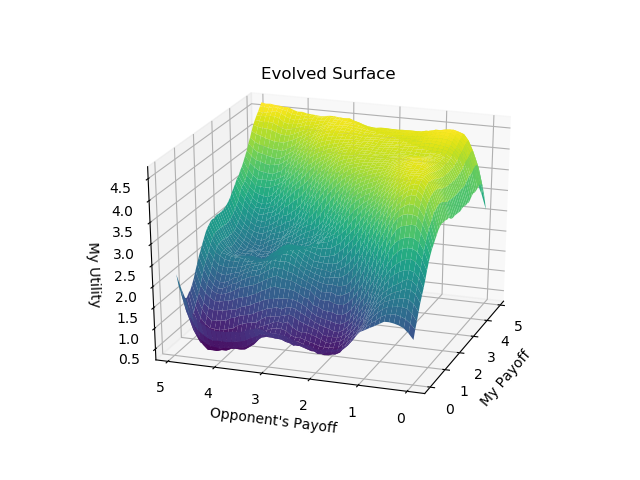
\includegraphics[scale=0.7]{resources/average_r_0_symmetric_evolved.png}
	\caption{An average of the surfaces evolved by symmetric-game, phenotype mutation when $\alpha = 0$.}
	\label{average_r_0_symmetric_evolved}
\end{figure}

\begin{figure}
	\centering
	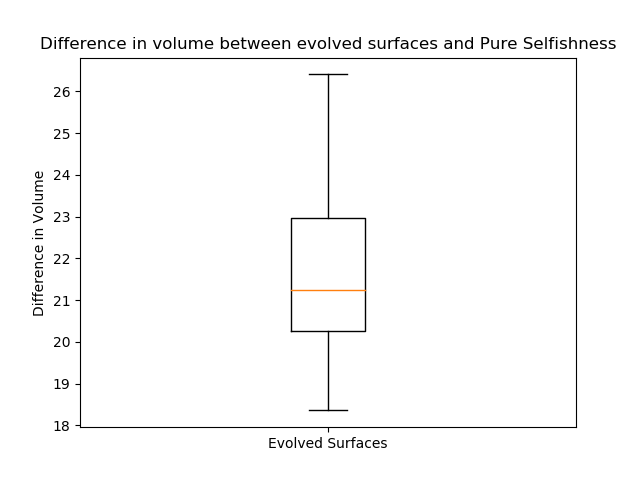
\includegraphics[scale=0.7]{resources/boxplot_volume_difference_symmetric_r_0.png}
	\caption{Volume-differences between evolved surfaces and Pure Selfishness; $\alpha = 0$.}
	\label{boxplot_volume_difference_symmetric_r_0}
\end{figure}

\np Performing similar analysis on the surfaces evolved when $\alpha \neq 0$ yields similar results.
The figure \ref{average_r_03_symmetric_evolved} shows the average evolved surface when $\alpha = 0.3$.
The volume-difference between this surface and the one shown in figure \ref{average_r_0_symmetric_evolved} is so small as to be negligible.
As before, we can also look at the volume differences between the surfaces produced by the simulation and the AW prediction.
Figure \ref{boxplot_volume_difference_symmetric_r_03} shows the distribution of these volumes, the volume-difference between the average surface and the AW prediction is 23.282.
Now that $\alpha$ is greater than zero and AW predicts some level of cooperation between individuals, our evolved surfaces are even more dissimilar to the AW prediction.

\begin{figure}
	\centering
	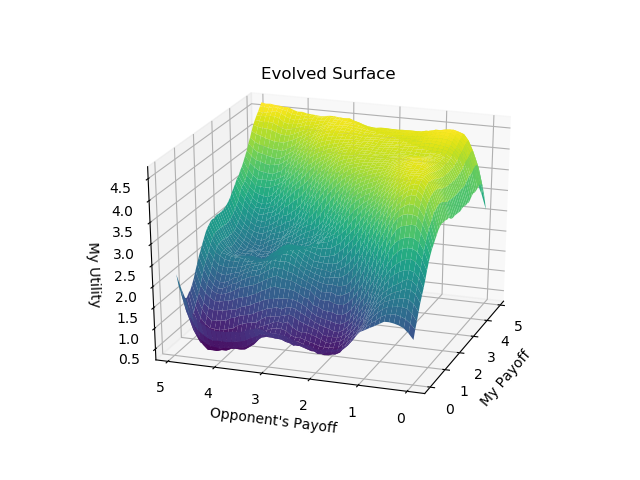
\includegraphics[scale=0.7]{resources/average_r_03_symmetric_evolved.png}
	\caption{An average of the surfaces evolved by symmetric-game, phenotype mutation when $\alpha = 0.3$.}
	\label{average_r_03_symmetric_evolved}
\end{figure}

\begin{figure}
	\centering
	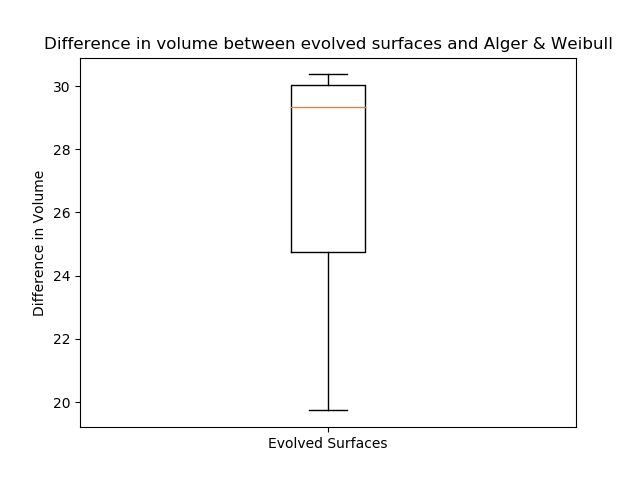
\includegraphics[scale=0.6]{resources/boxplot_volume_difference_symmetric_r_03.png}
	\caption{Volume-differences between evolved surfaces AW prediction; $\alpha = 0.3$.}
	\label{boxplot_volume_difference_symmetric_r_03}
\end{figure}


\np So, our evolved surfaces are not overly similar to the prediction made by AW surface in terms of volume-difference, but how do they fare in terms of fitness?
Figure \ref{linegraph_fitness_difference_increasing_epsilon} shows the difference in personal fitness earned by the evolved surface against the AW prediction as the proportion of the population  that is the evolved surface increases.
In this figure, a positive number on the \textit{y-axis} indicates that evolved surface has achieved a higher fitness increase than the AW prediction.
The downward slope of this figure indicates that when the AW prediction is the resident in a population and our average-evolved surface enters this population,
the evolved surface achieves a higher personal payoff than the prediction when the proportion of the population that is the evolved type is low.
As this proportion increases though, the fitness difference moves back in favour of the AW predication, and so our evolved surface will not be able to invade.
This is in agreement with AW's prediction.

\begin{figure}
	\centering
	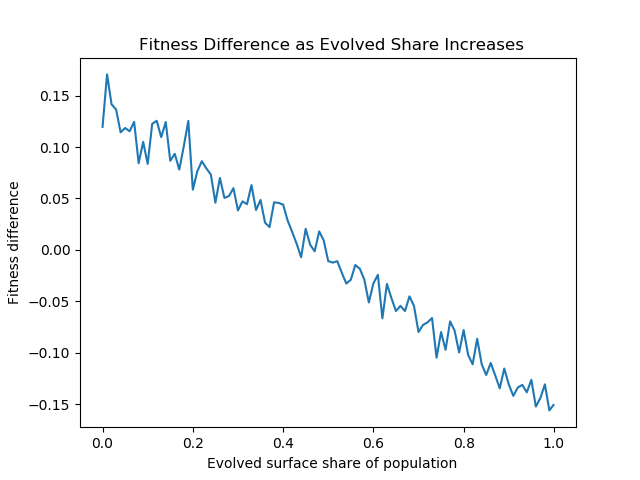
\includegraphics[scale=0.7]{resources/linegraph_fitness_difference_increasing_epsilon.png}
	\caption{Fitness difference between evolved surface and predicted surface; $\alpha = 0$.}
	\label{linegraph_fitness_difference_increasing_epsilon}
\end{figure}

\np Phenotype Mutation with symmetric games has not been able to recover the results of \citet{alger_generalization_2012}.
We did though, converge towards an interesting surface that performed reasonably well in fitness evaluation.
This well-performing surface allowed us to investigate the evolutionary stability of the AW prediction which we were not able to create a counter-example to. 
It is possible that this method of mutation has produced surfaces that are on their way to converging on an alternative evolutionary stable function.

\section{Symbolic Regression}

We now turn our attention to our second method of representing individuals.
We start with a randomly generated genome, and simulate evolution via the technique described.
In the case of symbolic regression, it is a little more difficult to give a general picture of the kinds of functions that evolved than it is in the phenotypic case.
Since small mutations in genome can lead to vastly different functions being generated by the grammar, it does not make sense to think of an average function that is generated,
but we can think about the kinds of functions that are generated.

\np Considering one group of ten simulations, where $\alpha = 0$, six of the evolved functions correspond exactly to pure selfishness, while two more are heavily slanted towards selfishness.
Finally, two of the resultant functions can be considered noise.
These results and the corresponding functions are displayed in figure \ref{barchart_fitness_earned_against_target_r_00}.
The dashed, threshold-line in this figure is the fitness earned by Pure Selfishness when playing against itself.

\np It can quickly be seen that functions $f$ and $g$ are poorest performing functions of the group.
This is makes sense when the functions themselves are considered: in generating a utility value neither function takes into account the player's payoffs.
It should also be noted that for completeness the full, unsimplified, evolved function is shown in the figure when some can be reduced.
For example, given that $r=\alpha=0$, functions $d$ and $h$ both reduce down to simply $my\_payoff$.
Another point to note is that functions $b$ and $i$, for example, result in exactly the same behaviour because the slopes of the resultant surfaces are equal.
The utility value generated by a particular function has no meaning if compared to the value generated by another individual.
Utility only carries weight when it is compared to another utility value of the same individual. 


\begin{figure}
	\centering
	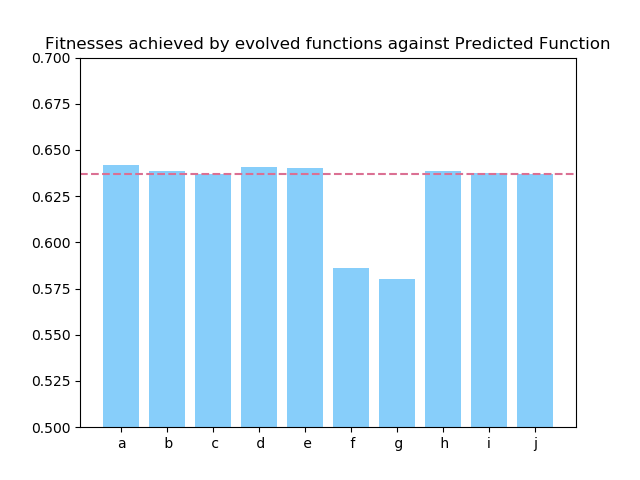
\includegraphics[scale=0.7]{resources/ylim_barchart_fitness_earned_against_target_r_00.png}
	{\tiny
	\begin{flalign*}
		a: r+my\_payoff*12.37-opponent\_payoff&\\
		b: my\_payoff+70.54&\\
		c: 47.17*my\_payoff-48.68&\\
		d: opponent\_payoff*r+my\_payoff+60.34*r*opponent\_payoff*20.72\\
		e: my\_payoff+r\\
		f: r*31.38\\
		g: 34.68+r\\
		h: my\_payoff+opponent\_payoff*my\_payoff*my\_payoff*opponent\_payoff*r\\
		i: my\_payoff-97.58\\
		j: my\_payoff+48.00\\
	\end{flalign*}
	}%
	\caption{Fitness earned by each evolved function when playing against AW prediction; $\alpha = 0$. In the evolved functions, r is used as a stand in for $\alpha$.}
	\label{barchart_fitness_earned_against_target_r_00}
\end{figure}

\np With no assortativity in the matching process, symbolic regression seems to converge towards the selfishness predicted by AW,
but we'll see now that things are a little more complicated when assortativity is introduced.

\begin{figure}
	\centering
	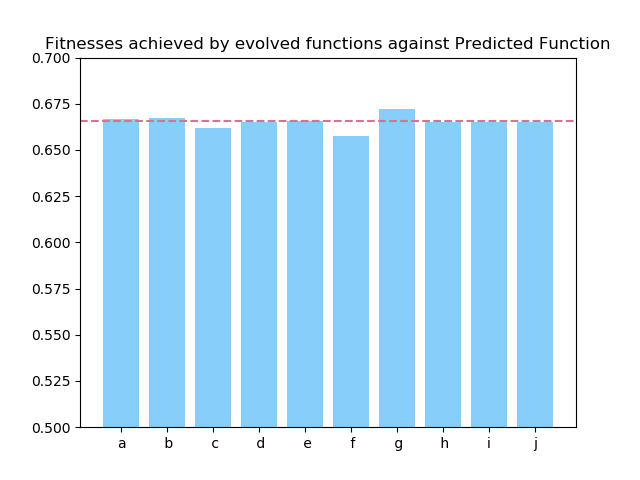
\includegraphics[scale=0.7]{resources/ylim_barchart_fitness_earned_against_target_r_06.png}
	{\tiny
		\begin{flalign*}
			a: r*opponent\_payoff+my\_payoff*05.89*r-my\_payoff*r+opponent\_payoff-opponent\_payoff\\
			b: r*opponent\_payoff-r+my\_payoff\\
			c: 03.02+46.57*54.25*78.80*my\_payoff\\
			d: my\_payoff+my\_payoff+opponent\_payoff\\
			e: r+r+r+r+r*opponent\_payoff+my\_payoff*r*r-r+opponent\_payoff+\\my\_payoff*my\_payoff*my\_payoff+my\_payoff*81.45+opponent\_payoff*\\42.48-r\\
			f: 11.03+my\_payoff\\
			g: opponent\_payoff-r*r+33.14-my\_payoff+26.75*opponent\_payoff*opponent\_payoff+13.71+83.53+\\opponent\_payoff-my\_payoff*my\_payoff*r-opponent\_payoff*02.65+my\_payoff+my\_payoff*\\56.95*my\_payoff+r-my\_payoff+my\_payoff-my\_payoff-my\_payoff+r+r*opponent\_payoff*r\\
			h: r+opponent\_payoff+r+01.11+my\_payoff*r*r*78.35*my\_payoff-r+r*74.62*opponent\_payoff\\
			i: my\_payoff-my\_payoff+opponent\_payoff+r-21.64+my\_payoff*r*my\_payoff\\
			j: opponent\_payoff+my\_payoff+my\_payoff+my\_payoff+opponent\_payoff\\
		\end{flalign*}
	}%
	\caption{Fitness earned by each evolved function when playing against AW prediction; $\alpha = 0.6$. In the evolved functions, r is used as a stand in for $\alpha$.}
	\label{barchart_fitness_earned_against_target_r06}
\end{figure}

\np Figure \ref{barchart_fitness_earned_against_target_r06} shows that while the simulations have not converged to functions that completely align with the AW prediction,
the behaviour of the individuals in fitness interactions is relatively similar.
Where the simulations has been unable to produce a function that exactly matches the AW prediction, the individuals have trended towards approximations.
Function $j$ is a good example of this.
When $\alpha = 0.6$, the AW function predicts that an individual who values their opponent's payoff with 0.6 the weight that they value their own will result in ESS play.
We can simplify function $j$ to the below:
{\small
\begin{flalign*}
	f(my\_payoff, opponent\_payoff) = 2\times opponent\_payoff+3 \times my\_payoff
\end{flalign*}
}%
\noindent Since we are only interested in the weights associated with each player's payoff, the above is equivalent to:
{\small
\begin{flalign*}
	f(my\_payoff, opponent\_payoff) = \frac{2}{3}\times opponent\_payoff+ my\_payoff
\end{flalign*}
}%

\noindent Which is a quite close approximation of the AW prediction.
This difficulty in converging to the exact AW prediction that arises when $\alpha \neq 0$, could be because the function we're attempting to evolve in this case is more complicated than finding an equivalent to pure selfishness.
There are just more ways to arrive at an equivalent of selfishness than there are at an equivalent of \ref{linearESSEquation}, and so we see the simulations more easily converge in the case when $\alpha = 0$.

\chapter{Asymmetric Games}\label{asymmetricGames}

\chapter{Discussion}\label{discussion}

 > The cause of weird divide in symmetric phenotype
 > whether evolved surfaces are candidate for ESS.

\paragraph{Phenotype Mutation: In it to win it}
\np The hypothesis is that this divide along the line of equality is a product of sampling only symmetric games.
In essence, when games are symmetric, each interaction that a resident and mutant engage in occurs across the line of equality.
Payoff points that are on the line of equality ($[a,a] \& [d,d]$) do not contribute to a difference in fitness, so can be ignored.
The other two payoff points in a given game are ($[b,c] \& [c,b]$), arbitrarily, let's assume that $b \geq c$.
So, since the point containing a and d contribute no difference to fitness, evolution will favour the outcome in which the individuals earns \textit{payoff b}.
By definition, this is always on the same side of the identity line, so that may explain the shape on the evolved functions.

\section{Games Matter}

\todo{Review this section after results are written to see where (if?) it fits}

One of the things that we learn by subjecting the described phenotype to evolution is that the kinds of games that are used to evaluate the fitness of individuals are important.
We begin with a model that uses only a single kind of game to evaluate the fitness of individuals.
Next we move to a conception of fitness that is an aggregation of individuals performance in many different kinds of games.
We explore this evaluation in the symmetric and asymmetric case in chapters \ref{symmetricGames} and \ref{asymmetricGames} respectively.

\paragraph{Single-Game Fitness Measure}
\np In \ref{experimentalFramework} we discuss an approach in which individual fitness is determined based off  how the types perform in one common kind of non-cooperative game, namely prisoner's dilemma.
Using the game structure defined in figure \ref{symmetricGame} we can construct a prisoner's dilemma by setting the following payoffs:
\begin{gather*}
	a = 3\\
	b = 0\\
	c = 4\\
	d = 1
\end{gather*}

\np When running simulations in which each type's fitness is determined by their expected payoff when playing the above game,
it becomes clear that only mutations that occur near to the payoff points ever lead to invasions. 
The payoff points are the four potential outcomes (in terms of payoffs for each player) of the game: (3,3), (0,4), (4, 0) \& (1, 1).
Plotted in figure \ref{prisoners_payoff_plot}.
\begin{figure}
	\centering
	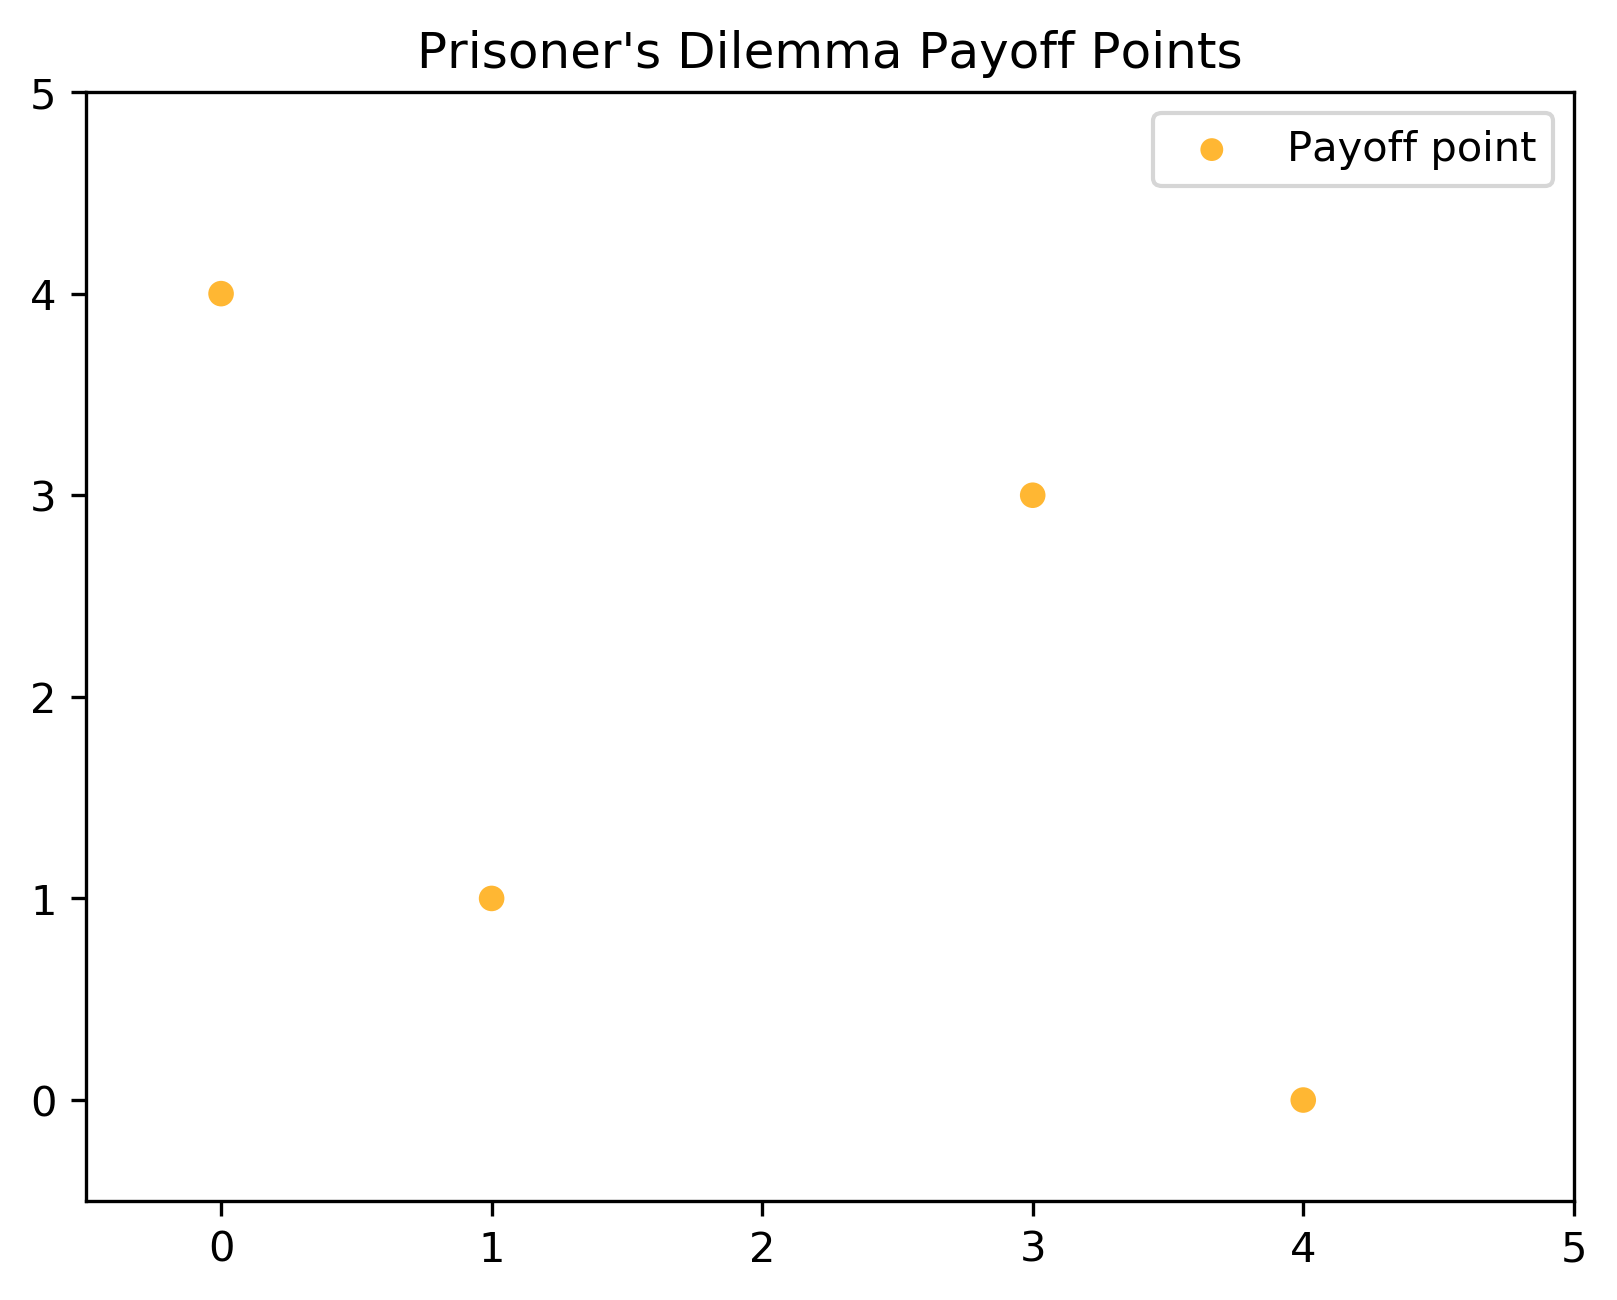
\includegraphics[scale=0.5]{resources/prisoners_dilemma_payoffs.png}
	\caption{The payoff points in a prisoner's dilemma game.}
	\label{prisoners_payoff_plot}
\end{figure}

\np The fact that limited invasions occur in this scenario makes sense when several facts about the model are considered:
\begin{enumerate}[label=(\alph*)]
	\item mutations can occur anywhere within the space and are small.
	\item the fitness of the individuals (resident and mutant) is equal in areas of the surface not affected by the mutation.
	\item for a mutant to invade, they must achieve a fitness \textit{greater} than that achieved by the resident - as opposed to greater than or equal to.	
\end{enumerate} 
\np
So, if a mutation occurs at the point (2, 2), given that this mutation has a relatively small radius, 
the expected payoff of the mutant will not differ from that of the resident because the mutation does not touch any of the payoff points.
Hence, the fitnesses are equal, and no invasion occurs.
Running simulations using this model results in `utility surfaces' that seem to have a evolved to play the prisoner's dilemma defined above,
rather than evolving towards a surface that is meaningful in general.

\todo{distance/fitness measure of prisoner's dilemma run}

\np So, while our source material tends to equivocate in regard to what kinds of games are played,
a dynamically evolving system shows that evaluating individual fitnesses using performance in only one kind of game 
does not generate meaningful results. Next, we focus on a  measure in which fitness is based upon the individual's aggregated performance across many games.

\paragraph{Many-Game Fitness Measure}
\np We move to a discussion of the results generated by simulations that measure fitness as an average of the payoff earned by individuals across many symmetric games.
Now, the games that individuals play in determining fitness contain payoffs as described in \ref{a_through_d}, where $a$ through $d$ are independent and identically distributed random variables.
Leading on from our note in the preceding that single-game fitness leads to an exorbitantly high number of mutations that do not lead to an invasion, analogously, 
localised mutations and randomly sampled games is computationally very inefficient. So, we first look at a more efficient sampling mechanism before discussing our main result.

\np Sampling many symmetric games creates a payoff-point plot that is symmetric about the line of equality and the line of equality is heavily sampled relative to the rest of the space.
This is because two of the four payoff points in each sampled game fall on the line of equality.
If we imagine the payoff-point plot (e.g. figure \ref{prisoners_payoff_plot}) as being a top-down view of one of our utility surfaces,
then we can randomly place a mutation amongst the sampled payoff-points to visualise the amount of waste that occurs when sampling like this.
Figure \ref{symmetric_payoff_plot} shows a randomly sampled mutation plotted amongst payoff-points of 40 randomly sampled games.
\begin{figure}
	\centering
	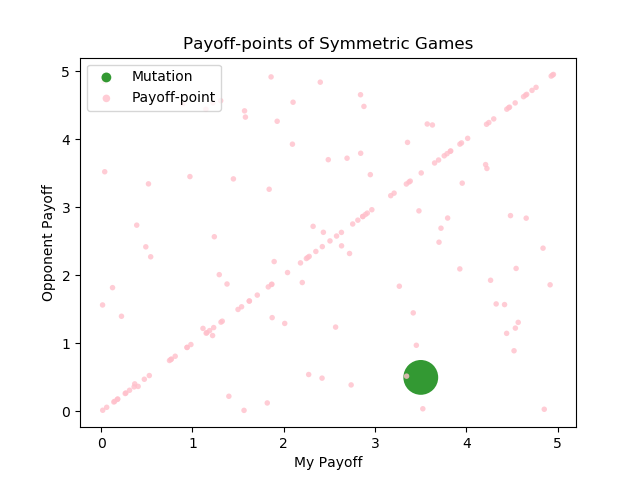
\includegraphics[scale=0.7]{resources/scatter_symmetric_mutation.png}
	\caption{Payoff-points of 40 randomly sampled games.}
	\label{symmetric_payoff_plot}
\end{figure}
We can see that of the 160 payoff points in the sample, only one occurred in the area of the mutation.
The rest of the payoff points will not contribute to a difference in fitness between the resident and mutant and so are a waste of computational resources.
We develop a more efficient sampling technique.
In this technique, two of the four payoff points in a symmetric-game still occur along the line of equality,
but the other two in each game are sampled from close to the mutation.
The payoffs $a$ through $d$ are sampled from the following, where $\mu$ is the centre of the mutation and $\delta$ is some constant linked to the radius of the mutation.
\begin{center}\label{local_a_through_d}	
	$a \sim U(0,\phi) \qquad a \in I$
	
	$b \sim \mu \pm U(0,\delta) \qquad b \in I$
	
	$c \sim \mu \pm U(0,\delta) \qquad c \in I$
	
	$d \sim U(0,\phi) \qquad d \in I$
\end{center}


\noindent Figure \ref{local_symmetric_payoff_plot} is an example of a sample of 40 games in which the payoffs are sampled using this technique.
It can be seen that payoff-points are now concentrated around the area that the mutation occurs so will contribute to a difference in fitness.
This technique means that every game will have at least one payoff-point that touches the mutation area.
This technique introduces no additional bias into the model: it is as if we freely sample payoffs from the whole space and then filter out the ones that do not have an effect on eventual fitness comparison.

\begin{figure}
	\centering
	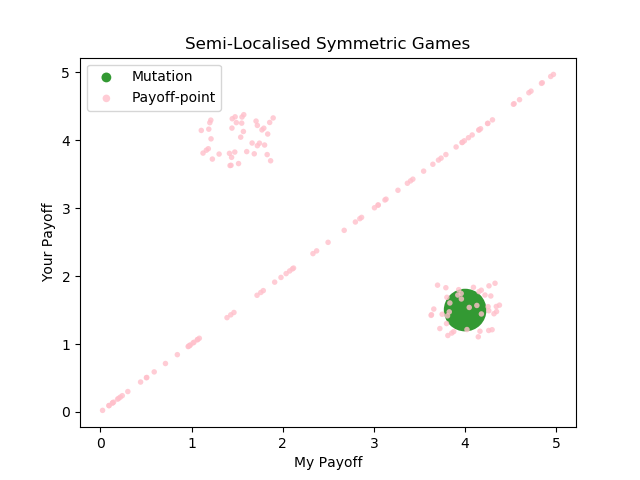
\includegraphics[scale=0.7]{resources/localised_symmetric_game_mutation.png}
	\caption{Payoff-points of 40 `locally' randomly sampled games.}
	\label{local_symmetric_payoff_plot}
\end{figure}

\chapter{Conclusion}


\todo{is this to speculative/waffley?}
Intuitively, the non-meaningful results achieve when sampling only one kind of game fit with our analogy of the utility function in some way representing the real-world preferences of some agent.\
In reality, agents face many more kinds of situations than just one instance of a prisoner's dilemma,
and so to generate a utility function that is potentially recognisable as one of a real-world agent the function will need to be resilient to many different situations.


\bibliography{thesis}
\bibliographystyle{apalike}

\end{document}